% Standalone TikZ figure: Multi-Objective Pareto Front
% For Chapter 7: Reward Function Engineering
\documentclass[tikz,border=10pt]{standalone}
\usepackage{tikz}
\usepackage{amsmath}
\usetikzlibrary{arrows.meta, positioning, shapes.geometric, calc, patterns, decorations.pathreplacing}

\begin{document}
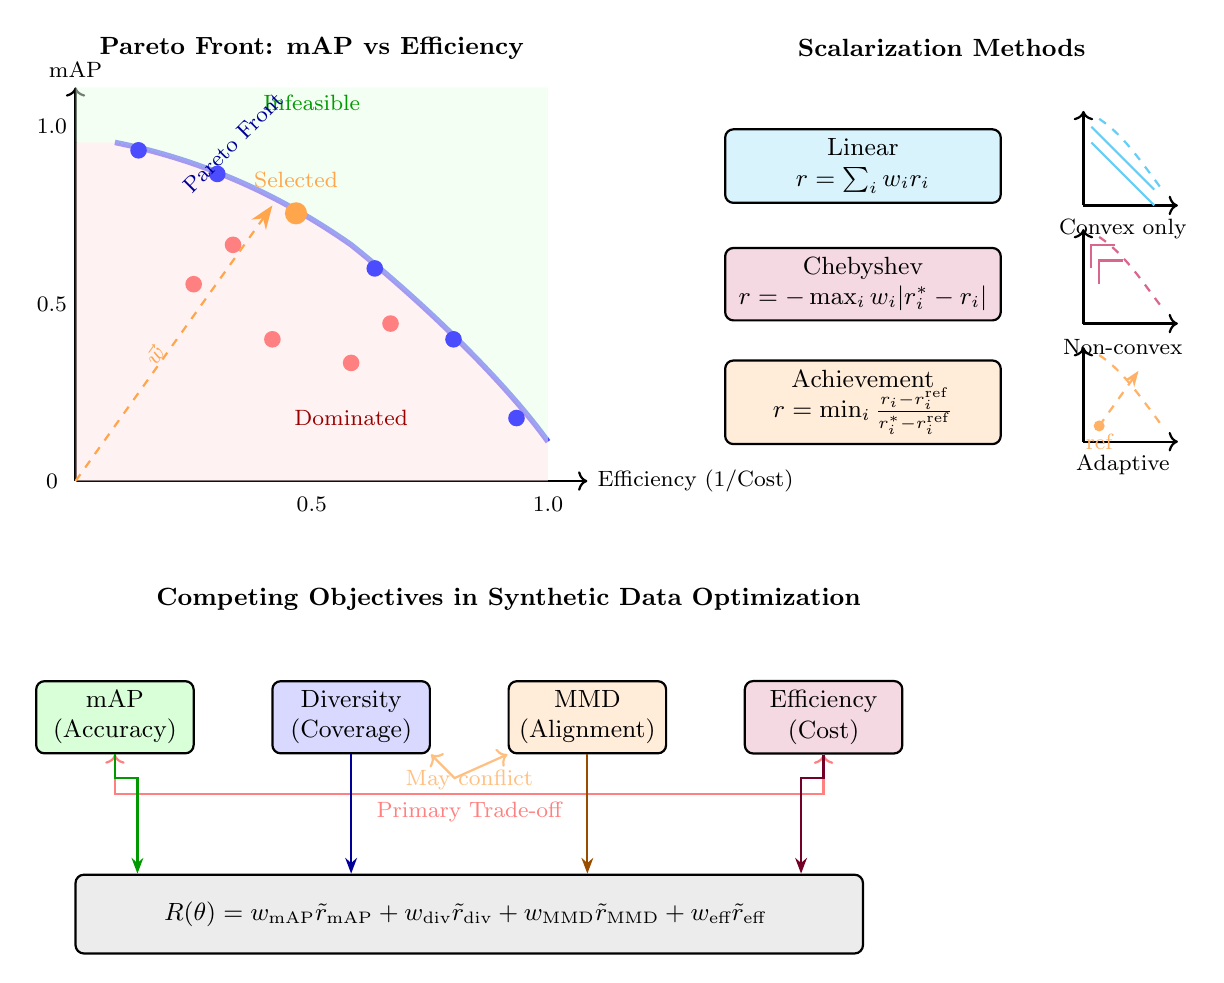
\begin{tikzpicture}[
    node distance=1.2cm and 1.5cm,
    every node/.style={font=\small},
    box/.style={rectangle, draw, thick, minimum width=2cm, minimum height=0.8cm, align=center, rounded corners=3pt},
    arrow/.style={-{Stealth[length=2mm]}, thick},
    label/.style={font=\footnotesize},
    title/.style={font=\bfseries\small}
]

% ============ PARETO FRONT (LEFT) ============
\node[title] at (3, 5.5) {Pareto Front: mAP vs Efficiency};

% Axes
\draw[thick, ->] (0, 0) -- (0, 5) node[above, label] {mAP};
\draw[thick, ->] (0, 0) -- (6.5, 0) node[right, label] {Efficiency (1/Cost)};

% Axis labels
\node[label] at (-0.3, 4.5) {1.0};
\node[label] at (-0.3, 2.25) {0.5};
\node[label] at (-0.3, 0) {0};
\node[label] at (3, -0.3) {0.5};
\node[label] at (6, -0.3) {1.0};

% Pareto front curve
\draw[thick, blue!70, line width=2pt]
    (0.5, 4.3) .. controls (1.5, 4.1) and (2.5, 3.7) .. (3.5, 3) .. controls (4.5, 2.2) and (5.5, 1.2) .. (6, 0.5);

% Dominated region (shaded)
\fill[red!10, opacity=0.5]
    (0.5, 4.3) .. controls (1.5, 4.1) and (2.5, 3.7) .. (3.5, 3) .. controls (4.5, 2.2) and (5.5, 1.2) .. (6, 0.5) -- (6, 0) -- (0, 0) -- (0, 4.3) -- cycle;

% Non-dominated region
\fill[green!10, opacity=0.5]
    (0.5, 4.3) .. controls (1.5, 4.1) and (2.5, 3.7) .. (3.5, 3) .. controls (4.5, 2.2) and (5.5, 1.2) .. (6, 0.5) -- (6, 5) -- (0, 5) -- (0, 4.3) -- cycle;

% Pareto optimal points
\fill[blue!70] (0.8, 4.2) circle (3pt);
\fill[blue!70] (1.8, 3.9) circle (3pt);
\fill[blue!70] (2.8, 3.4) circle (3pt);
\fill[blue!70] (3.8, 2.7) circle (3pt);
\fill[blue!70] (4.8, 1.8) circle (3pt);
\fill[blue!70] (5.6, 0.8) circle (3pt);

% Dominated points
\fill[red!50] (1.5, 2.5) circle (3pt);
\fill[red!50] (2.5, 1.8) circle (3pt);
\fill[red!50] (3.5, 1.5) circle (3pt);
\fill[red!50] (2, 3) circle (3pt);
\fill[red!50] (4, 2) circle (3pt);

% Labels
\node[label, green!60!black] at (3, 4.8) {Infeasible};
\node[label, red!60!black] at (3.5, 0.8) {Dominated};
\node[label, blue!60!black, rotate=45] at (2, 4.3) {Pareto Front};

% Weight vector arrow
\draw[thick, orange!70, -{Stealth[length=3mm]}, dashed] (0, 0) -- (2.5, 3.5);
\node[label, orange!70, rotate=54] at (1, 1.6) {$\vec{w}$};
\fill[orange!70] (2.8, 3.4) circle (4pt);
\node[label, orange!70, above] at (2.8, 3.6) {Selected};

% ============ SCALARIZATION METHODS (RIGHT) ============
\node[title] at (11, 5.5) {Scalarization Methods};

% Linear scalarization
\node[box, fill=cyan!15, minimum width=3.5cm] (linear) at (10, 4) {Linear\\$r = \sum_i w_i r_i$};

% Chebyshev scalarization
\node[box, fill=purple!15, minimum width=3.5cm] (cheby) at (10, 2.5) {Chebyshev\\$r = -\max_i w_i|r_i^* - r_i|$};

% Achievement function
\node[box, fill=orange!15, minimum width=3.5cm] (asf) at (10, 1) {Achievement\\$r = \min_i \frac{r_i - r_i^{\text{ref}}}{r_i^* - r_i^{\text{ref}}}$};

% Small diagrams for each
% Linear - straight lines
\begin{scope}[shift={(12.8, 4)}]
    \draw[thick, ->] (0, -0.5) -- (0, 0.7);
    \draw[thick, ->] (0, -0.5) -- (1.2, -0.5);
    \draw[cyan!60, thick] (0.1, 0.5) -- (0.9, -0.3);
    \draw[cyan!60, thick] (0.1, 0.3) -- (0.9, -0.5);
    \draw[cyan!60, thick, dashed] (0.2, 0.6) .. controls (0.5, 0.4) and (0.7, 0.1) .. (1, -0.3);
    \node[label] at (0.5, -0.8) {Convex only};
\end{scope}

% Chebyshev - L-shaped contours
\begin{scope}[shift={(12.8, 2.5)}]
    \draw[thick, ->] (0, -0.5) -- (0, 0.7);
    \draw[thick, ->] (0, -0.5) -- (1.2, -0.5);
    \draw[purple!60, thick] (0.1, 0.2) -- (0.1, 0.5) -- (0.4, 0.5);
    \draw[purple!60, thick] (0.2, 0) -- (0.2, 0.3) -- (0.5, 0.3);
    \draw[purple!60, thick, dashed] (0.2, 0.6) .. controls (0.5, 0.4) and (0.7, 0.1) .. (1, -0.3);
    \node[label] at (0.5, -0.8) {Non-convex};
\end{scope}

% Achievement - reference point
\begin{scope}[shift={(12.8, 1)}]
    \draw[thick, ->] (0, -0.5) -- (0, 0.7);
    \draw[thick, ->] (0, -0.5) -- (1.2, -0.5);
    \fill[orange!60] (0.2, -0.3) circle (2pt);
    \node[label, orange!60] at (0.2, -0.5) {ref};
    \draw[orange!60, thick, dashed, -{Stealth[length=2mm]}] (0.2, -0.3) -- (0.7, 0.4);
    \draw[orange!60, thick, dashed] (0.2, 0.6) .. controls (0.5, 0.4) and (0.7, 0.1) .. (1, -0.3);
    \node[label] at (0.5, -0.8) {Adaptive};
\end{scope}

% ============ TRADE-OFF EXAMPLES (BOTTOM) ============
\node[title] at (5.5, -1.5) {Competing Objectives in Synthetic Data Optimization};

% Objective boxes
\node[box, fill=green!15] (obj1) at (0.5, -3) {mAP\\(Accuracy)};
\node[box, fill=blue!15] (obj2) at (3.5, -3) {Diversity\\(Coverage)};
\node[box, fill=orange!15] (obj3) at (6.5, -3) {MMD\\(Alignment)};
\node[box, fill=purple!15] (obj4) at (9.5, -3) {Efficiency\\(Cost)};

% Trade-off indicators
\draw[thick, red!50, <->] (obj1.south) -- ++(0, -0.5) -| (obj4.south);
\node[label, red!50] at (5, -4.2) {Primary Trade-off};

\draw[thick, orange!50, <->] (obj2.south east) -- ++(0.3, -0.3) -- (obj3.south west);
\node[label, orange!50] at (5, -3.8) {May conflict};

% Composite reward formula
\node[box, fill=gray!15, minimum width=10cm, minimum height=1cm] (composite) at (5, -5.5) {
    $R(\theta) = w_{\text{mAP}} \tilde{r}_{\text{mAP}} + w_{\text{div}} \tilde{r}_{\text{div}} + w_{\text{MMD}} \tilde{r}_{\text{MMD}} + w_{\text{eff}} \tilde{r}_{\text{eff}}$
};

% Arrows to composite
\draw[arrow, green!60!black] (obj1.south) -- ++(0, -0.3) -| ($(composite.north west) + (0.8, 0)$);
\draw[arrow, blue!60!black] (obj2.south) -- ++(0, -0.6) -| ($(composite.north) + (-1.5, 0)$);
\draw[arrow, orange!60!black] (obj3.south) -- ++(0, -0.6) -| ($(composite.north) + (1.5, 0)$);
\draw[arrow, purple!60!black] (obj4.south) -- ++(0, -0.3) -| ($(composite.north east) + (-0.8, 0)$);

\end{tikzpicture}
\end{document}
